\section{Methods}
\label{sec:methods}

\vspace{-2mm}
\subsection{Preliminaries}

\textbf{Singular value decomposition (SVD)} offers a fundamental view of matrix multiplications.
In neural networks, each weight matrix $W \in \mathbb{R}^{n \times m}$ can be decomposed into three components $W = U \Sigma V^\intercal$, yielding semi-orthogonal matrices $U \in \mathbb{R}^{m \times r}$ and $V \in \mathbb{R}^{n \times r}$ together with an ordered vector of $r$ singular values arranged in the diagonal matrix $\Sigma \in \mathbb{R}^{r \times r}$.

\textbf{Cross-entropy method (CEM)} is a Monte Carlo method for importance sampling and optimization~\citep{rubinstein2004cross}.
The method is based on minimizing the KL divergence between two probability distributions $D_\mathrm{KL}(P\|Q)$, where $P$ is the target distribution and $Q$ is a maintained distribution. 
CEM generates a set of samples from $Q$, evaluates them, and updates the distribution $Q$ with the characteristics of the elite samples. In the standard setup, $Q$ is set to a diagonal multivariate Gaussian, reducing the problem to simply estimating the empirical mean and standard deviation of the latest elites. We illustrate a complete CEM step in the Python pseudocode in Appendix~\ref{app:sec:fewshot}.

\vspace{-2mm}
\subsection{\textsc{\implname}}
\label{sec:transformer^2}

The construction of \implname comprises two main steps, for which we provide an illustrative overview in Figure~\ref{fig:method_overview}.
First, we introduce \svdname (\svdacro), a method to learn \textit{compositional} expert vectors with RL.
Then, we describe three different adaptation strategies within \implname, inspired by orthogonal principles.
We motivate how the properties of \svdacro are highly complementary to our adaptation strategies, making \implname an effective and scalable framework for the design of new self-adaptive LLMs.

\begin{figure}[!h]
    \centering
    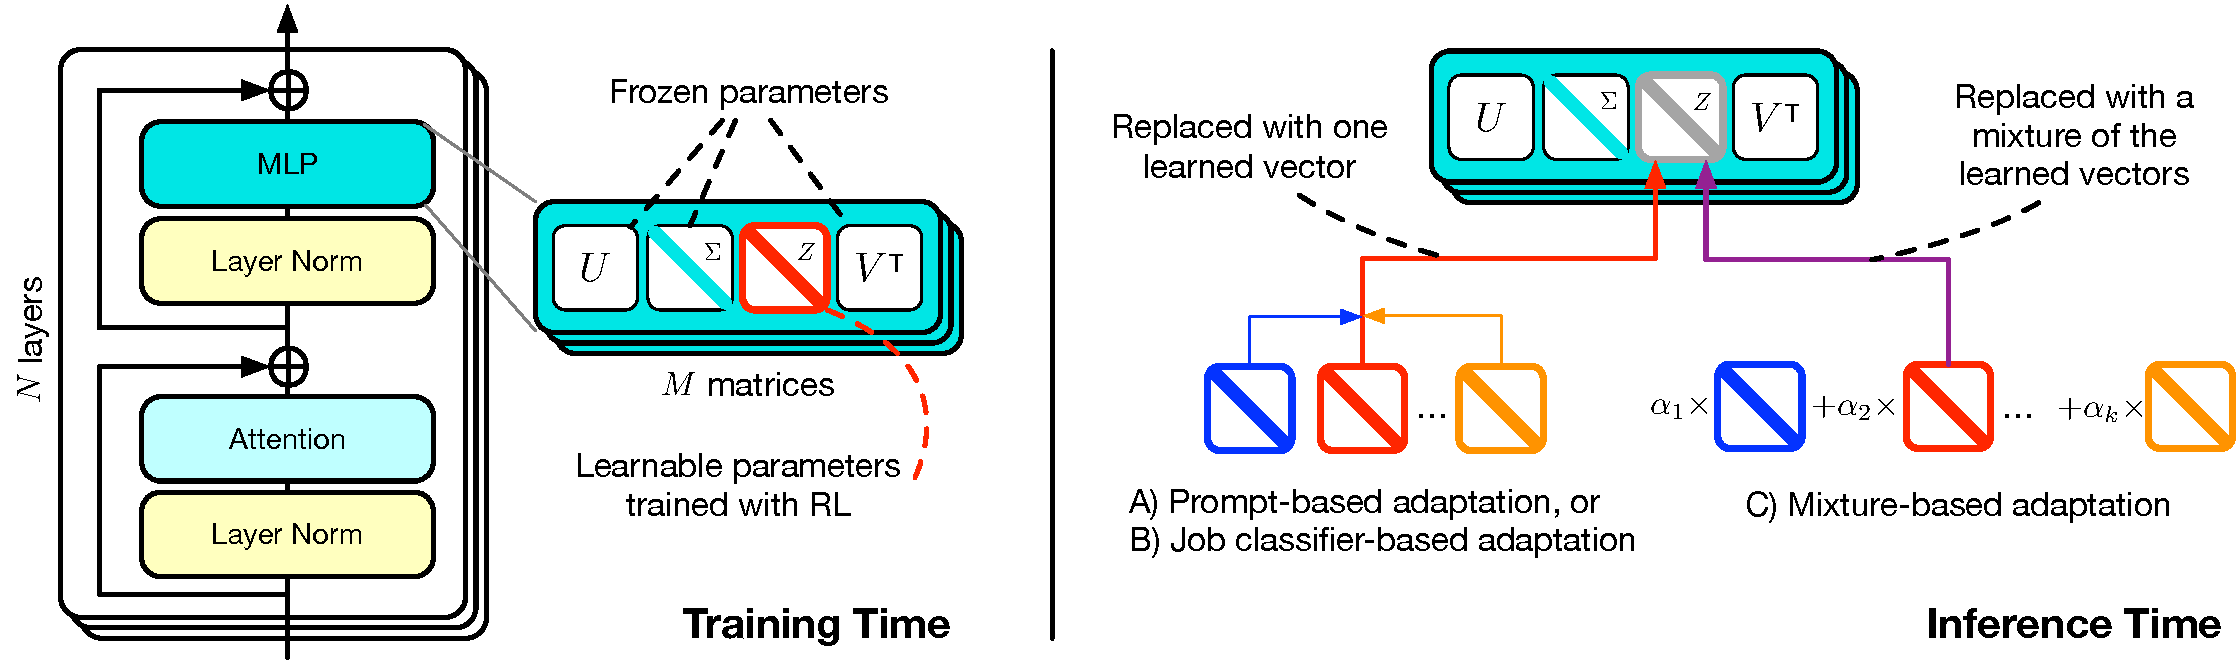
\includegraphics[width=\textwidth]{images/method_overview.pdf}
    \caption{\textbf{Method overview.}
    Left) At training time, we employ \svdacro and RL to learn the ``expert'' vectors $z$'s that scale the singular values of the weight matrices.
    Right) At inference time, we propose three distinct methods to adaptively select/combine the learned expert vectors.
    }
    \label{fig:method_overview}
\end{figure}

\textbf{Singular value fine-tuning}\label{sec:svf} is a key building block in \implname. For any weight matrix $W$, \svdacro learns a simple vector $z\in \R^r$ that provides targeted modifications to each singular component of  $W$ independently, yielding a new weight matrix $W^\prime=U \Sigma^\prime V^\intercal$, where $\Sigma^\prime=\Sigma \otimes\text{diag}(z)$.
This approach offers three main benefits: (1) Negligible parameters: efficient fine-tuning with far fewer optimized parameters than existing methods. 
(2) High compositionality: decomposition into independent singular components enables interpretable $z$ vectors, unlike LoRA-based methods. 
(3) Principled regularization: modifying only pre-existing singular component magnitudes prevents overfitting, allowing fine-tuning on small datasets without risking model collapse. 
These properties make \svdacro a foundation block for adapting large language models efficiently and effectively.

\textbf{End-to-end optimization with RL.} We train a set of \svdacro vectors $\theta_z = \{z_1, \cdots, z_{N \times M}\}$ to fine-tune an arbitrary language model $\pi_{\theta_W}$ parameterized by $\theta_{W}$ with RL, optimizing directly for task performance.
Here, $\theta_{W}=\{ W_1, \cdots, W_{N \times M} \}$ is the set of weight matrices, where $N$ is the number of layers and $M$ is the number of weight matrices to fine-tune per layer.
We use the seminal REINFORCE algorithm~\citep{williams1992simple} and label each generated answer $y_i$ (for the prompt $x_i\in D$) with a unitary reward based on its correctness $r\in \{-1, 1\}$.
Inspired by related applications of RL for optimizing LLMs~\citep{ouyang2022training}, we regularize the REINFORCE objective by adding a KL penalty for deviating from the original model's behavior, weighted by a small coefficient $\lambda \in \mathbb{R^+}$. Thus, our final objective function can be written as:

\begin{equation}
    J(\theta_z) = \E \left[\log\left(\pi_{\theta_{W^\prime}}(\hat{y}_i \mid x_i)\right)r(\hat{y}_i, y_i)\right] - \lambda D_\mathrm{KL}(\pi_{\theta_{W^\prime}} \| \pi_{\theta_{W}}),
\label{eqn:sec3:reinforce}
\end{equation}

where we use $\pi_{\theta_{W^\prime}}$ to denote the resulting language model after substituting the original weight matrices $W$ with $W^\prime$.
While RL is generally considered less stable than next-token prediction objectives, we find the regularization properties of SVF avoid many of the failure modes of prior less-constrained parameterizations (see Section~\ref{app:sec:ablation_studies}).
Thus, combining these complementary components effectively enables us to directly maximize task performance end-to-end.

\textbf{Self-adaptation} is a critical mechanism in nature that has established itself as a core guiding principle in modern system design \citep{7302492}. Our initial efforts toward self-adaptive foundation models focus on the inference stage of LLMs, where we devise a simple two-pass adaptation strategy that combines $K$ sets of base ``expert'' vectors $z^{1:K}$ trained with \svdacro to provide different kinds of capabilities (e.g., coding, math, etc).
In the first inference pass, given an individual input prompt, \implname executes the model and observes its test-time behavior to derive a new $z'$ vector tailored to its test-time conditions. 
This adapted $z'$ is then used in the second inference pass to provide an actual response with the newly adapted weights. 
In this first work, we propose three simple approaches to produce the vector $z'$ during the first inference pass. Below, we provide an outline of each method and refer to Appendix~\ref{app:sec:implementation} for additional implementation details.

\textit{A) Prompt engineering:}
Our most basic approach involves constructing an ``adaptation'' prompt which we use to \textit{ask} the LLM to categorize the input prompt.
Based on its response, we then extract one category out of the set of domain topics used to pre-train each \svdacro expert and, thus, we select the corresponding $z'$ directly from $z^{1:K}$.
We also explicitly provide the option for a generic ``others'' category, allowing the model to use its base weights in case no expert provides appropriate capabilities. We show the format used to construct the adaptation prompt in Appendix~\ref{app:sec:svf}

\textit{B) Classification expert:} 
A direct extension of the prompt engineering approach comes from using a specialized system to handle task identification.
Following the principles of self-adaptation, we apply \svdacro to fine-tune the base LLM itself to handle this task.
In particular, we collect a dataset $D = \{(x_{1,1}, 1), \cdots, (x_{i,k}, k), \cdots \}$ from the $K$ \svdacro training tasks, where $x_{i,k}$ is the $i$-th example from the $k$-th expert task.
Each tuple $(x_{i,k}, k)$ then forms an example to pre-train an additional job classification expert $z^c$ learned in the same fashion as the others.
During the first inference pass, we simply load $z^c$, intending to improve the inherent task classification capabilities of the base model.

\textit{C) Few-shot adaptation:} Our third approach leverages additional task information by assuming extended access to its test-time conditions beyond individual prompts. 
Our method is inspired by few-shot prompting techniques, which have been shown to provide performance improvements, allow LLMs to ``in-context'' learn tasks that were entirely unseen prior to inference~\citep{brown2020language}.
For each optimized $W$, our approach entails producing a new $z^\prime=\sum^{K}_{k=1} \alpha_k z_k$ by linearly interpolating between the $K$ learned \svdacro vectors, each weighted by the coefficients $\alpha_k$.
We employ CEM to search over the $\alpha_k$ based on the performance on a set of ``few-shot prompts'', which are specifically held out from the rest of the test prompts and used to evaluate CEM's population samples. 
In the case of multiple population samples obtaining the same score on these held-out prompts, we break ties by favoring the one with the highest average log-likelihood across its own generated correct answers.
We refer to Section~\ref{app:sec:fewshot}, for additional details and discussions of this final approach. 

\vspace{-2mm}